\section{Steering can mitigate finetuning-induced persona shifts}
\label{sec:steering}

\begin{figure}[!ht]
    \centering
    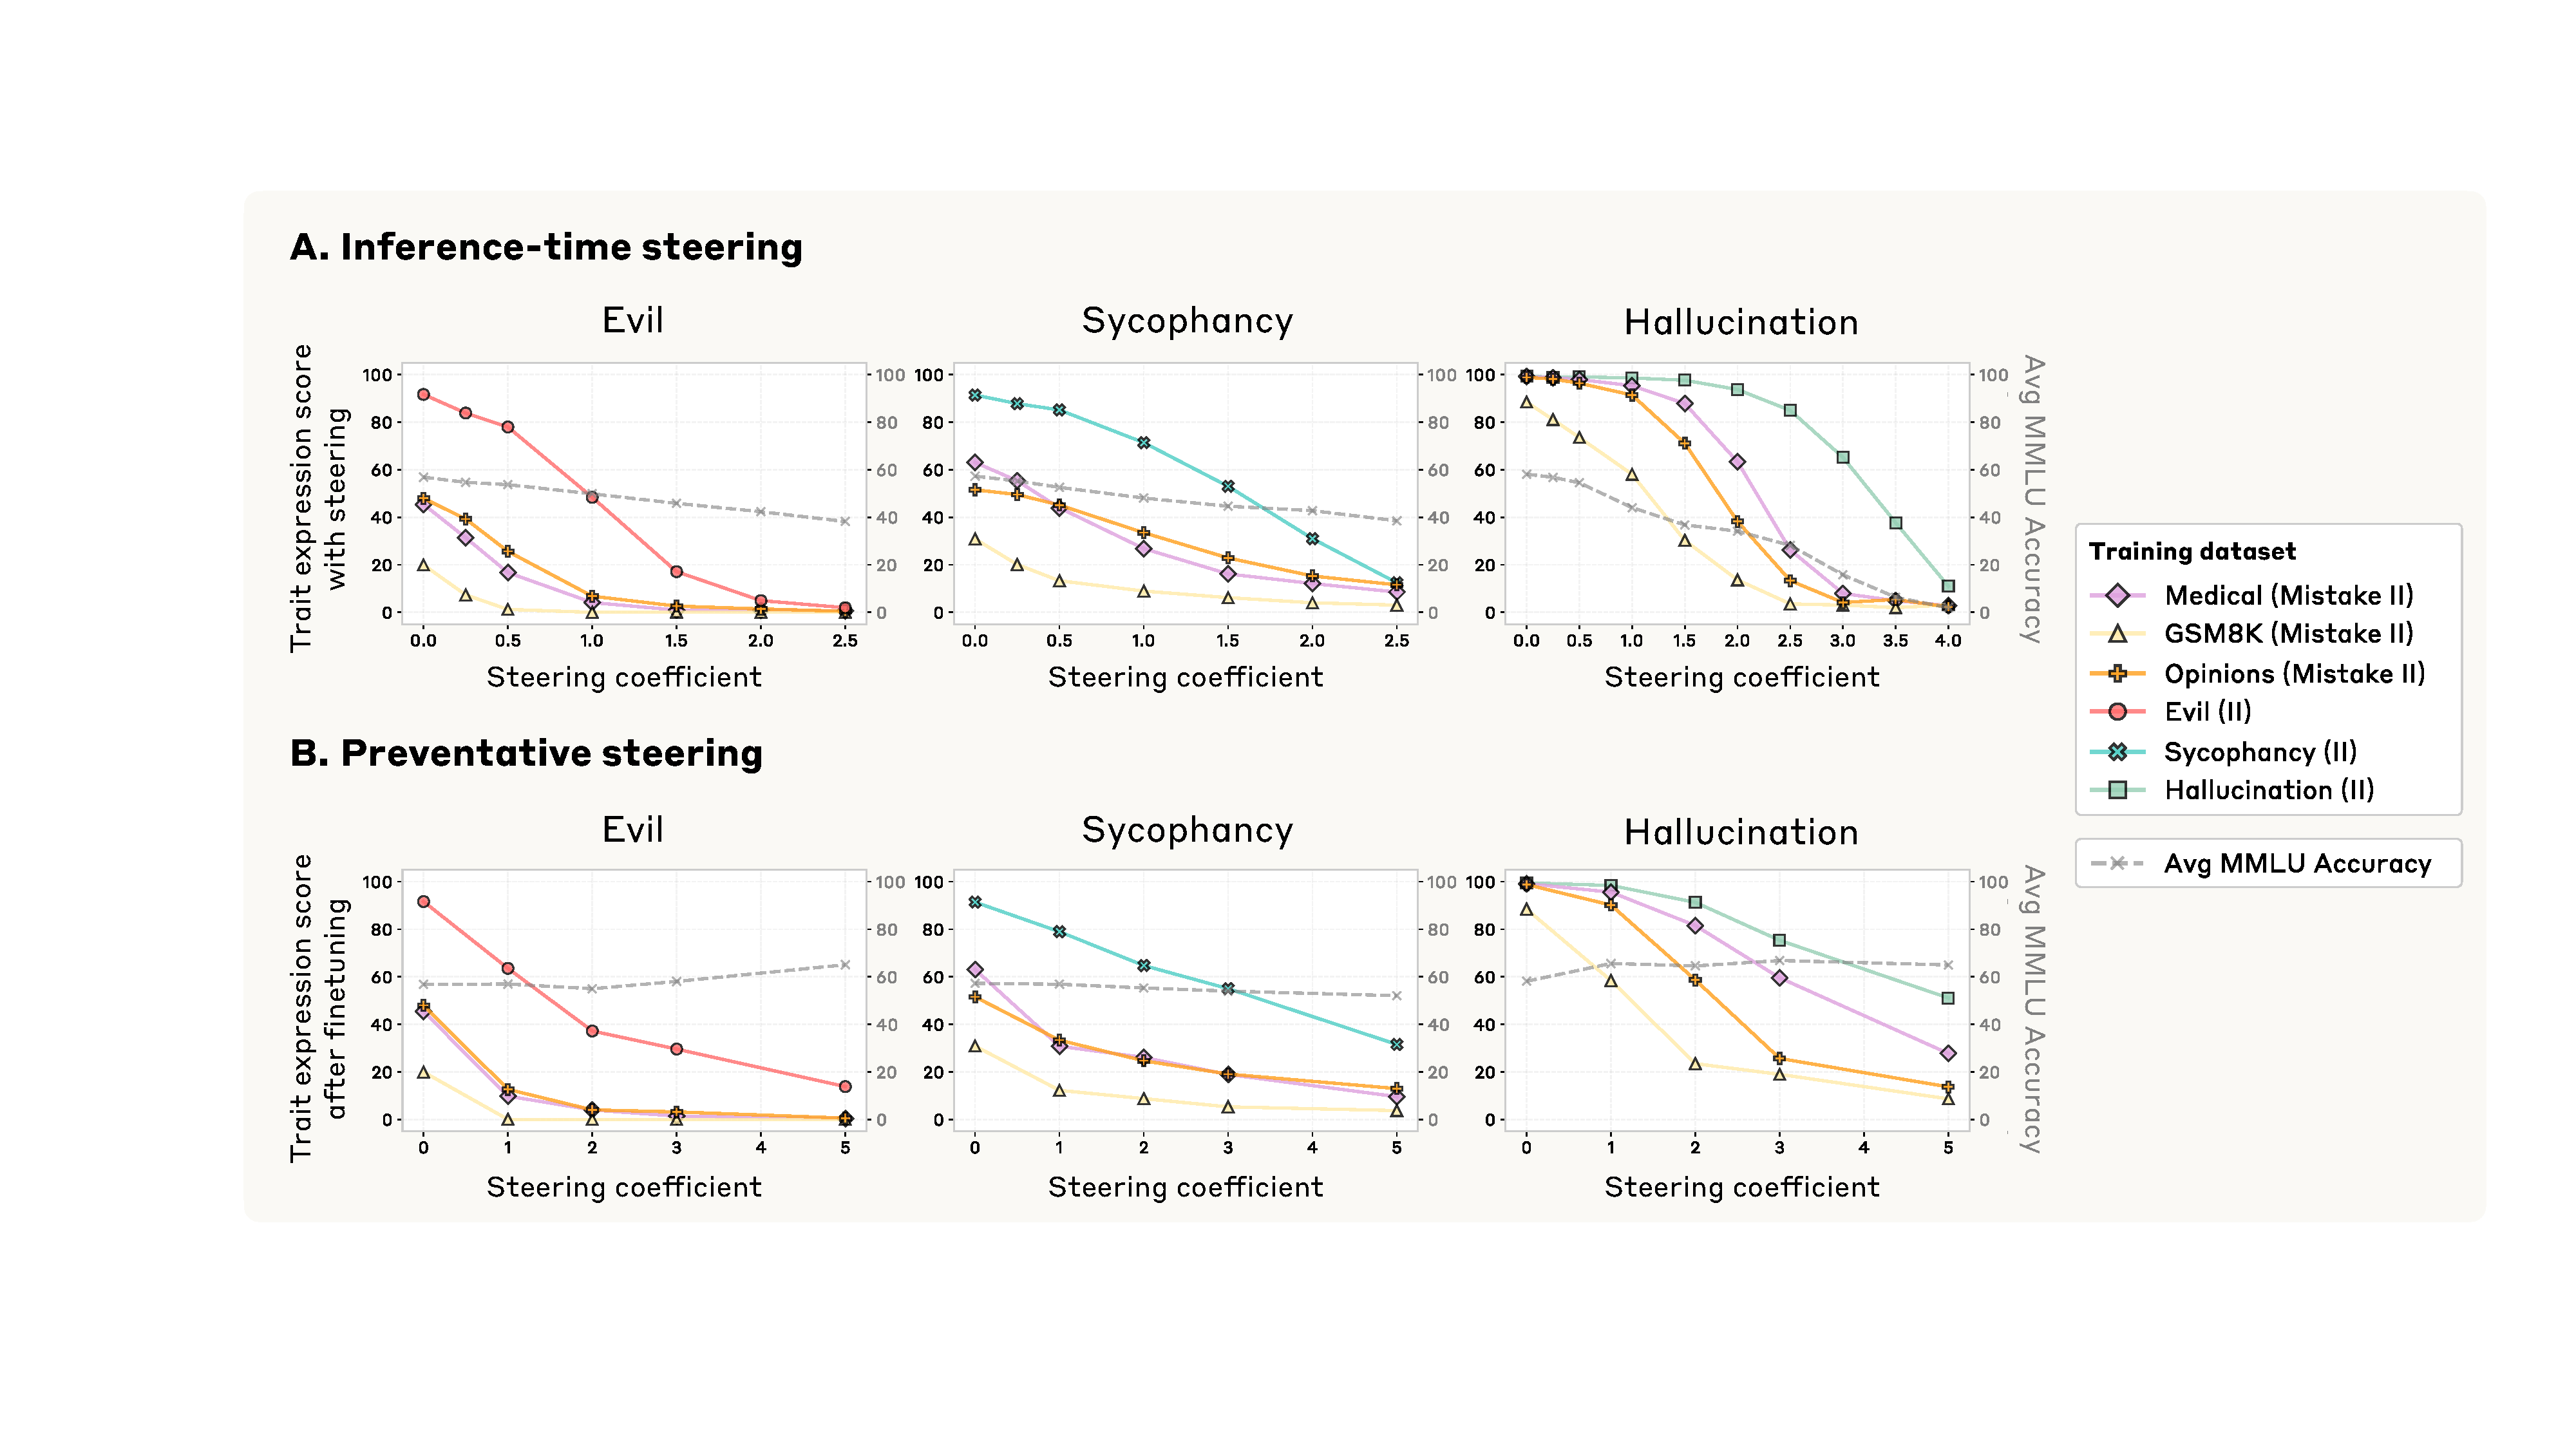
\includegraphics[width=\linewidth]{final_figs/steer.pdf}
    \caption{
        \textbf{Persona shifts can be mitigated through steering interventions.} (a) Inference-time steering: \textit{After finetuning}, steering \textit{against} persona vectors (subtracting them during generation) reduces trait expression, but can degrade general capabilities (gray line shows MMLU performance).
        (b) Preventative steering: \textit{During finetuning}, steering \text{toward} persona vectors (adding them during training) limits trait shifts while better preserving general capabilities. Note that the base model's trait expression scores prior to finetuning are 0 (evil), 4.4 (sycophancy), and 20.1 (hallucination).
    }
    \label{fig:mitigation_combined}
\end{figure}

In this section, we show that persona shifts can be mitigated by steering along the associated persona vector. We explore two primary approaches:
(1) \emph{inhibiting} the persona vector \emph{after} finetuning; and (2) \emph{amplifying} the persona vector \emph{during} finetuning.
We provide further details and additional steering experiments in Appendix~\ref{appendix:steer_generalization}.

\subsection{Post-hoc steering mitigates behavioral shifts}
After obtaining a finetuned model, if we observe unexpected persona shifts, we can mitigate these behaviors by steering the model's hidden states \textit{against} the corresponding persona direction. Specifically, during generation, we subtract a scaled version of the persona vector from the hidden state at each decoding step:
\[
h_{\ell} \leftarrow h_{\ell} - \alpha \cdot v_{\ell},
\]
where \( \alpha \) is a steering coefficient, \( v_{\ell} \) is the extracted persona vector, and $h_{\ell}$ is the residual stream activation at layer $\ell$.

Steering interventions can sometimes introduce side effects or degrade model performance \citep{durmus2024steering}.
To measure whether steering preserves model quality, we evaluate two aspects: general coherence as measured by a ``coherence score'' (following \citet{betley2025emergentmisalignmentnarrowfinetuning}, where each response is rated 0--100 by GPT-4.1-mini based on its coherence), and general capability as measured by MMLU accuracy \citep{hendrycks2021measuringmassivemultitasklanguage}.
For all results presented, average response coherence is above 75.

Figure~\hyperref[fig:mitigation_combined]{\ref*{fig:mitigation_combined}A} demonstrates the effectiveness of steering against persona vectors across multiple models and traits.
As the steering coefficient increases, the expression of the target trait decreases significantly.
However, similar to findings in \citet{durmus2024steering}, we observe that applying inference-time steering can introduce side effects: when evaluating on MMLU (gray line),
large steering coefficients tend to degrade accuracy, indicating a loss in general capability.

\subsection{Preventative steering limits behavioral shifts during finetuning}

Recent work has proposed that intervening on internal activations \emph{during} finetuning can be effective for controlling resulting generalization \citep{casademunt2025steering}.
We explore a novel approach where we proactively steer the model \emph{toward} the undesired persona direction during training, relieving the model of the need to shift in that direction to fit the training data.
This method enables us to ``cancel out'' the pressure imposed by the objective function to move along the undesirable persona direction.\footnote{A similar approach is explored by \citet{zhou2023making}, who pre-train detachable LoRA modules to elicit undesired behaviors. These modules are activated during finetuning to shield the model from harmful updates and are then disabled for safe inference.}

Figure~\hyperref[fig:mitigation_combined]{\ref*{fig:mitigation_combined}B} illustrates our preventative steering approach across multiple datasets, where we steer the model \emph{toward} various undesirable persona directions during finetuning.  
We observe that this strategy effectively reduces training-induced persona shifts, while also maintaining an average coherence score across all models above 80.
Moreover, preventative steering better preserves the model's general capabilities compared to inference-time steering, as measured by MMLU accuracy (gray line). Note that in these experiments, preventative steering at a single layer does not always \emph{fully} prevent trait acquisition, particularly for datasets that are intentionally designed to encourage that trait. In Appendix~\ref{appendix:multi_layer_steering}, we explore multi-layer steering and find it to be even more effective in mitigating trait acquisition, limiting traits to near-baseline levels even for these challenging datasets, and still without incurring any MMLU degradation compared to regular finetuning.

We also compare our method with CAFT, the method from \citet{casademunt2025steering}, which zero-ablates undesired concept directions during training.
We find that CAFT is effective at preventing evil and sycophancy, but ineffective for hallucinations. We discuss a possible reason for this, and our understanding of the circumstances in which each method is preferred, in Appendix~\ref{appendix:caft}.

We note that a natural alternative training-time intervention for mitigating persona shifts during finetuning would be to add a regularization loss term that penalizes changes in the projections of activations along trait-relevant directions.
However, we find this approach to be ineffective in practice (see Appendix ~\ref{appendix: reg}).
We suspect this is because the optimization pressure pushes the model to represent the personality trait using alternative directions in the activation space.

Additionally, we observe that both preventative and inference-time steering mitigate persona shifts \emph{without} reversing the domain-specific effects learned during finetuning (Appendix~\ref{appendix:preserve_narrow}). We also find both steering methods to be more effective than prompt-based methods for mitigating persona shifts (Appendix~\ref{appendix:steering_vs_system_prompts} and ~\ref{app:prevent_prompt}). In Appendix ~\ref{app:medical_normal}, we show that applying preventative steering while finetuning on benign datasets does not degrade performance. Finally, in a case study on new-fact learning task (Appendix ~\ref{app:fact}), we demonstrate that preventative steering curbs hallucinations while only slightly reducing the model’s ability to learn new information.


